\message{ !name(report.tex)}\documentclass[]{article}
\usepackage{amsmath}
\usepackage{amsfonts}
\usepackage{amssymb}
\usepackage{mathtools}
\usepackage{fullpage}
\usepackage{graphicx}
\usepackage{fixltx2e}
\usepackage{listings}
\usepackage{color}
\usepackage{setspace} 
\usepackage{multirow}
\usepackage{tikz}
\usetikzlibrary{calc,decorations.markings,shapes.misc,fadings,decorations.pathreplacing}


\tikzset{cross/.style={cross out, draw, 
         minimum size=2*(#1-\pgflinewidth), 
         inner sep=0pt, outer sep=0pt}}

\definecolor{mycolor1}{RGB}{204,51,63}
\definecolor{mycolor2}{RGB}{0,160,176}
\definecolor{mycolor3}{RGB}{217,206,178}
\long\def\/*#1*/{}
\newcommand{\HRule}{\rule{\linewidth}{0.5mm}}

\definecolor{dkgreen}{rgb}{0,0.6,0}
\definecolor{gray}{rgb}{0.5,0.5,0.5}
\definecolor{mauve}{rgb}{0.58,0,0.82}

\lstset{frame=tb,
  language=C,
  aboveskip=3mm,
  belowskip=3mm,
  showstringspaces=false,
  columns=flexible,
  basicstyle={\small\ttfamily},
  numbers=none,
  numberstyle=\tiny\color{gray},
  keywordstyle=\color{blue},
  commentstyle=\color{dkgreen},
  stringstyle=\color{mauve},
  breaklines=true,
  breakatwhitespace=true
  tabsize=3
}

\onehalfspacing

\begin{document}

\message{ !name(report.tex) !offset(-3) }

\begin{titlepage}
\begin{center}

\vspace*{1.0cm} 
{\huge \bfseries The properties of quantum dots formed by interstitial Mn\textsubscript{\emph{i}}\textsuperscript{2+} ions in p-i-n resonant tunneling diodes \\[0.4cm] }
\vspace{0.8cm} 

% Author and supervisor
\begin{minipage}{0.4\textwidth}
\begin{flushleft} \large
\emph{Author:}\\
Timothy \textsc{Fogarty}\textsuperscript{1}* 
\end{flushleft}
\end{minipage}
\begin{minipage}{0.4\textwidth}
\begin{flushright} \large
\emph{Supervisor:} \\
Dr.~Oleg \textsc{Makarovsky}\textsuperscript{1}
\end{flushright}
\end{minipage}
\\[0.8cm]
\textsuperscript{1}School of Physics \& Astronomy, University of Nottingham, Nottingham NG7 2RD, United Kingdom

*To whom correspondence should be addressed, \texttt{pcytf@nottingham.ac.uk}

\vspace{0.8cm} 
{\large \today}
\vspace{0.8cm} 

\begin{abstract}
Lorem ipsum dolor sit amet, consectetur adipiscing elit. Nulla at nisl a tellus pretium porta. Nunc dapibus mi egestas, elementum quam ut, pellentesque justo. Quisque nec purus quis lectus venenatis posuere. Vivamus bibendum neque at ante eleifend, id adipiscing felis volutpat. Proin ultrices quam nec dui consequat lacinia. Morbi lectus lectus, fringilla nec aliquet vitae, pharetra quis felis. Phasellus adipiscing faucibus bibendum. Nam aliquet felis vel lobortis accumsan. Cras ut ullamcorper lectus, ac ultricies ligula. Proin sed molestie metus, sed condimentum sem. Suspendisse in pellentesque augue. Morbi elit arcu, pharetra ac justo ac, sodales accumsan nisi. Pellentesque augue nulla, consectetur a urna porttitor, sodales malesuada purus. Fusce sit amet enim egestas, tincidunt nisl at, bibendum ante. Pellentesque dignissim ante quis auctor mollis.
\end{abstract}



\vfill

\textbf{Project source code available at:}

github.com/TimFogarty/GaAs-Potentials


% Bottom of the page


\end{center}
\end{titlepage}

\tableofcontents
\newpage
\section{Introduction}
\subsection{The rise of the MOSFET}
Computers are composed of logic gates. These logic gates are the physical implementation of Boolean functions $f:B^n \rightarrow B$, $B=\{0,1\}$ \cite{elements}. That is, logic gates are functions that take as input $n$ truth values and output one truth value. As such, computers are a physical implementation of a two-element Boolean algebra. Sheffer showed NAND and NOR gates are both functionally complete---any logic gate could be created by a network of NAND or NOR gates alone \cite{elements}. So to create a computer, many NAND gates must be connected together. Doing this requires the ability to switch and amplify electrical signals. Switching means flipping bits, and is necessary to implment Boolean functions. Amplification is used to ensure electrical signals don't attenuate and die as they propagate through a large number of logic gates. 

The transistor is an electrical component which can both switch and amplify electrical signals \cite{Guide to state-of-the-art electron devices}. Modern computers use MOSFETs (metal-oxide-semiconductor field-effect transistors) to implement logic gates. Transistors have three terminals. In MOSFETs current flows between two terminals, the \emph{source} and the \emph{drain}, and is modulated by the third, the \emph{gate}. The gate is made of polycrystalline silicon (historically a metal was used instead) and an oxide such as SiO$_2$. It acts as a capacitor. The source and drain are made of a doped semiconductor such as Silicon or Gallium Arsenide. Between the source and drain and perpendicular to the gate is the \emph{channel}, which is made of a semiconductor substrate doped differently to the source and drain. If the MOSFET is built on a p-type semiconductor, electrons travel from the source through the channel to the drain. This is an n-channel or nMOS transistor. Conversly, a transistor built on an n-type semiconductor would be called a p-channel or pMOS transistor. In the pMOS, the channel current would be made of holes and the current would flow from drain to source.

n-channel and p-channel MOSFETs are used together to implement logic gates. This is known as CMOS (complementary metal-oxide-semiconductor) technology. Many CMOS circuits can be placed on a single semiconductor chip, known as an \emph{integrated circuit}. For over 40 years, the width of MOSFETs have decreased by $\sim 0.7$ times every 2--3 years. In 1970, MOSFETs were 10 $\mu$m wide \cite{}. In 2012, they were 22 nm wide \cite{}. Because of this decline in MOSFET size, the number of transistors on integrated circuits have approximately doubled every 2 years. This trend of the number of components on integrated circuits doubling every 2 years was described in 1965 by Gordon Moore \cite{} and has since become known as Moore's Law. The decline in MOSFET size means that the gate capacitance can decrease. A smaller capacitance results in a shorter switching time and a lower switching power \cite{Guide to state-of-the-art electron devices}. The increase in the number of MOSFETs on integrated circuits have paved the way for parallel processing. Thus Moore's law causes an increase in speed, an increase in parallel processing capabilities, a decrease in power usage \cite{}, and a decrease in cost \cite{original moore}.

\subsection{Quantum limits of the MOSFET}
It has been suggested that this exponential growth of the density of transistors in CMOS circuits will not continue indefinitely. This is becasue there are well known physical limits to computation. The Bekenstein bound uses entropy to describe a limit on the information that can be processed by a finite region of space with a finite energy \cite{,}. The acceleration of the universe has been considered with the Bekenstein bound to put a universal limit on computation \cite{}. The lower bound to the energy required to change one bit is defined by the Second Law and is known as the Shannon-von~Neumann-Landauer expression, $E_{bit} \geq E_{SNL} = k_BT\ln 2$ \cite{}. Moreover, the physical limits of a theoretically perfect computer have been defined by the speed of light $c$, Planck's constant $h$, and the gravitational constant $G$ \cite{}. However, the most immediate limiting factor to Moore's law is that as MOSFETs become smaller, they will be disrupted by quantum effects \cite{,}.

In quantum tunnelling, electrons or holes have a non-zero probability of penetrating a potential barrier through which they classically would not have been able to move. With oxide layers thinner than 2 nm, carrier wavefunctions penetrate through the oxide and create a gate current \cite{thesis}. This leakage occurs in the channel, source, and drain regions \cite{thesis} and impairs the performance of CMOS circuits \cite{,}. Gate leakage could possibly be reduced by using high-$\kappa$ materials, such as HfO$_2$ \cite{}. However, another issue is band-to-band tunnelling. In this case carriers leak between n-type and p-type regions.

fundementally the size of MOSFETs are limited by Heisenberg's uncertainty principle, $\Delta x\Delta p \geq \hbar$ \cite{}. For a transistor operating at $E_{SNL}$
\begin{align}
x_{min} =& \frac{\hbar}{\Delta p} \\
=& \frac{\hbar}{2m_eE_{SNL}} \\
=& \frac{\hbar}{2m_ek_BT\ln 2} \\
=& 1.5~\text{nm} \qquad \text{($T = 300$ K)}
\end{align}
CMOS devices are currently made using the 22 nm node which specifies an nMOS transistor with a gate length of 9 nm \cite{}. Therefore CMOS circuits are close to their quantum mechanical limits.

\subsection{Probing the quantum nature of semiconductors}

As MOSFETs approach their physical limits, research is looking for ways to replace MOSFETs. Two areas of research are quantum computation and spintronics. Quantum computing seeks to use quantum entanglement effects to make quantum logic gates \cite{}. It has been successful in providing algorithms such as Shor's quantum algorithm for the discrete logarithm and Grover's quantum search algorithm. These algorithms are faster than their classical counterparts. However, quantum computation has seen slow progress in hardware due to the difficulty of trapping and measuring electrons or photons \cite{}. Spintronics (spin transport electronics) seeks to use not only the charge but also the spin of the electron in creating electronic devices \cite{}. Spintronic transistors \cite{Electronic analog of the electro‐optic modulator}, spintronic logic gates \cite{nature}, and spintronic integrated circuits \cite{http://arxiv.org/abs/1112.2746} have been proposed. spin-dependent transport of electrons in semiconductors has been demonstrated\cite{,}, as has a spintronic transistor \cite{,}.

Quantum dots (QDs) are semiconductor nanostructures that confine electrons in 3 dimensions \cite{}. Being able to confine electrons has possible applications in spintronics \cite{}, quantum computation \cite{qbook}, and nanophotonics \cite{4th}. Therefore, the study of quantum dots may contribute to finding a replacement for MOSFETs and the extension of Moore's Law. Many methods for the fabrication of QDs have been demonstrated such as nanolithography, colloidal synthesis, and self-assembly. Recently, laser annealing has been used to diffuse interstitial Mn$_i^{2+}$ ions from p-type (GaMn)As across the p-i interface in a p-i-n resonant tunnelling diode \cite{1,2,3,4}. Magnetotunnelling spectroscopy has shown that this forms quantum dots \cite{}. In p-type Ga$_{1-x}$Mn$_x$As, Mn is the dopant which replaces Ga atoms in the lattice. However, when $x > 2\%$ interstitial manganese, Mn$^{2+}_i$, forms in the center of the zincblende unit cell. 

This investigation implements a numerical model of blah. The potential landscapes created by the simulation were Fourier transformed. The transform showed that the quantum dots were Lorentzian in shape. The full width at half maximum (FWHM), $w$, of the quantum dots were shown to be related to the distance,$d$ from the plane of Mn ions, $w = 2.43d$. This is in agreement with blah. Moreover, the 2D investigation showed that quantum dots are not always circularly symmetric, they can be elongated. This is in agreement with blah. 

\section{Theory}

\subsection{Doping}

\subsection{Interstitial ions}

\subsection{The potential due to a finite line of uniform charge}
We search for the potential on a parallel line at a distance $d$ from a line of uniform charge of length $l$. Suppose the line of charge is composed of charges of inifinitesimal length. Then the potential at a point $d$ from that line is
\begin{equation}
V = \int \frac{1}{4\pi\epsilon_0}\frac{\text{d}q}{r}.
\end{equation}
Now, $\text{d}q = \lambda\text{d}x$ (where $\lambda$ is the charge density) and $r = \sqrt{x^2 + d^2}$. Therefore,
\begin{align}
V = & \frac{1}{4\pi\epsilon_0} \int_{-a}^{b}\frac{\lambda \text{d}x}{\sqrt{x^2+d^2}}\\
= & \frac{\lambda}{4\pi\epsilon_0} \ln \left(\frac{b+\sqrt{b^2+d^2}}{-a+\sqrt{a^2+d^2}}\right)
\end{align}
where $x = -a$ and $x = b$ at the boundaries of the line of charge (see Fig.~\ref{uniformpotentialdiagram}). Now the potential landscape defined over n points is
\begin{equation}\label{uniformeq1d}
V(x_i) = \sum_{i=1}^n\frac{\lambda}{4\pi\epsilon_0} \ln \left(\frac{b_i+\sqrt{b_i^2+d^2}}{-a_i+\sqrt{a_i^2+d^2}}\right)
\end{equation}
where $a_i = l - x_i$ and $b_i = l + x_i$. This function was implemented in MATLAB. The script was tested against a numerical model based on Eq.~\ref{poteq} and they were found to be in agreement. The shape of the uniform potential can be seen in Fig~\ref{uniformplot}.

\begin{figure}
\centering
\begin{tikzpicture}[scale=2]
\draw [red, thick, dashed] (4,0) --(2,-2);

\draw [thick, |-|] (0,0) --(6,0);

\node [thick, cross=4pt] at (2,-2) {};
\node [above] at (0,0.1) {$x=-a$};
\node [above] at (6,0.1) {$x=b$};
\draw [thick, dashed] (2,0) --(2,-2);
\draw (1.75,0) --(1.75,-0.25);
\draw (1.75,-0.25) --(2,-0.25);  
\node [thick, cross=4pt] at (2,0) {}; 
\node [above] at (2,0.1) {$x = 0$};
\shade[ball color=mycolor1] (4,0) circle(0.12);  
\node [above] at (4, 0.1) {C};
\node [above left] at (2,-2) {P};
\node [left] at (2,-1) {$d$};

\node [below right] at (3,-1) {$r$};
\end{tikzpicture}
\caption{The potential is calculated at point P. We integrate along the position $x \in [-a,b]$ of charge segments C. $x = 0$ at the point at which $r = d$.\label{uniformpotentialdiagram}}
\end{figure}

\begin{figure}
\centering
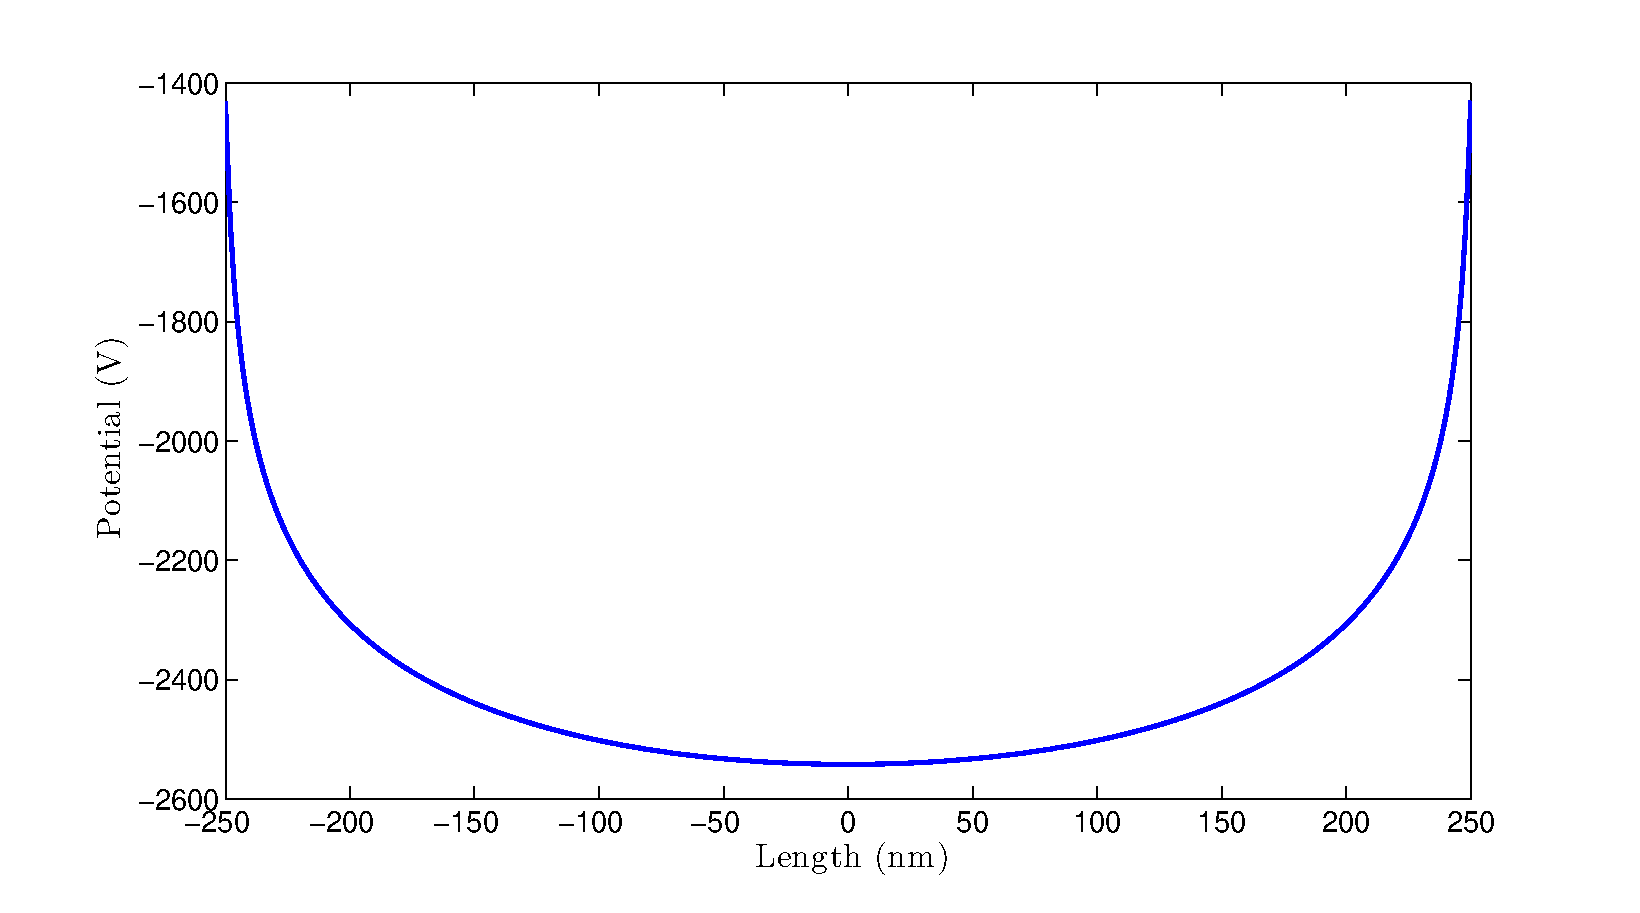
\includegraphics[width=\textwidth]{1d_Uniform_Potential.eps}
\caption{Eq.~\ref{uniformeq1d} was implemented in MATLAB. This is the potential at a distance 1 nm from a 500 nm line of uniform charge with charge density $\lambda = 6.4 \times 10^{11}$ Cm$^{-1}$. This was compared to a numerical simulation of 200 equally spaced charges over 500 nm. They were found to match. \label{uniformplot}}
\end{figure}

\subsection{The potential due to a disc of uniform charge}

\subsection{Fourier transforms}

\section{Method}

\subsection{The 1D investigation}

\subsubsection{Modelling the potential landscape}
\begin{equation}\label{poteq}
V(x) = \sum_{i=1}^n \frac{1}{4\pi\epsilon}\frac{2e}{r_i(x)}
\end{equation}

\begin{equation}
r_i(x) = \sqrt{d^2 + (x-C_i)^2}
\end{equation}

\subsubsection{The elimination of edge effects}

\subsection{The 2D investigation}

\subsubsection{Modelling the potential landscape}

\subsubsection{The elimination of edge effects using the potential due to uniform charge}

\subsection{Optimization of code}
Efficient code is important for large models. With large models, such as the 2D potential landscape simulations, efficient code can shave hours off of run time, leaving more time for analysis or more scope for bigger simulations. Moreover, models should be scalable. i.e. the algorithms in the models should have as low a comuptational complexity as possible. For example, $\mathcal{O}(n\log n)$ algorithms are favoured over $\mathcal{O}(n^2)$ algorithms because larger simulations will run much faster. An asymptotic analysis of algorithms is beyond the scope of this work, but run time was tested regularly and taken as an indicator of algorithmic efficiency. This section contains techniques the author found useful for improving the effieciency of MATLAB code.

\subsubsection{Vectorization}\label{sec:vectorization}
MATLAB is built on top of the Linear Algebra Package (LAPACK) and the Basic Linear Algebra Subprograms (BLAS) \cite{,}. These libraries operate on matrices using fast block algorithms \cite{}. Thus MATLAB is highly optimized for matrix and vector operations \cite{}. Generally, loops should be refactored into matrix operations where possible. This process is called \emph{vectorization} and results in faster, shorter, and more elegant code \cite{}. For example, an early version of the 1D potential landscape computation was this:

\lstset{language=Matlab}  
\begin{lstlisting}
for i = 1:length(x)
    for j = 1:length(chargePos)
        xPotential(i) = xPotential(i) - ...
            (1/(4*pi*epsilon0*epsilon))*((2*e)/(((d^2+(x(i)-chargePos(j))^2)^0.5)*10^-9));
    end
end
\end{lstlisting}
Vectorization yielded an improvement in efficiency and elegance. It can also be seen that extracting \texttt{const = (1/(4*pi*epsilon0*epsilon*10\textasciicircum -9))} out of the loop body meant fewer calculations per iteration. This also caused a speed-up.

\begin{lstlisting}
for i = 1:nDataPoints
    xPotential(i) = sum(const./(sqrt( d^2 + (x(i)-chargePos).^2)));
end
\end{lstlisting}
It is also worth noting all arrays were preallocated as resizing arrays each iteration can be computationally expensive.

\subsubsection{Refactoring functions}\label{sec:refactoringFunctions}
Function files provide a good way to abstract and modularize often-used code. To begin with, the main routine of computing the potential landscapes was abstracted into a function file. However, when functions are called in MATLAB, the arguments are passed into the function as whole objects, not pointers to the location of the objects in memory. Thus functions can be ineffiecient when they take a large amount of data as arguments. This is because all the data need to be copied into another space in memory. This performance loss could be mitigated by using MATLAB's \texttt{lib.pointer} class, and passing a pointer into the function. However, in this case, the author opted not to place the main routine within a function and to place the routine within the body of the main script instead. Therefore, no data must be copied and no pointers are necessary. This caused a large speed-up.

\subsubsection{Parallelization}
The outer \texttt{for} loop in the 2D algorithm seemed a good candidate for parallelization using \texttt{parfor}. These \texttt{parfor} loops require that each iteration is independent of the others. This is the case with the potential landscape algorithm. It is possible to see a linear speed-up with \texttt{parfor} \cite{}. 

During parallelization, MATLAB must assign iterations to the thread pool, and pass variables to each worker. This creates some overhead not present in single threaded algorithms. To make the extra overhead worth it, each iteration must be sufficiently computationally intensive. 

Attempting the parallelization over a pool of six workers resulted in a run time $\sim2$ times \emph{greater} than the unparallelized algorithm. It is possible that each iteration, although intensive, is not intensive enough to overcome the \texttt{parfor} overhead. Hence, the single threaded algorithm was used in this model. However, if a simulation with more charges and/or a greater area was attempted, parallelization may be advisable.

\subsubsection{Refactoring loops into C with MEX-files}
As mentioned in Section~\ref{sec:vectorization}, MATLAB is highly optimized for matrix operations. However, it is not as efficient at implementing loops as C. Given that the calculation of the 2D potential landscape uses nested loops, the calcualtion would be more efficient in C than in MATLAB.

C files can be built into binary \textbf{M}ATLAB \textbf{ex}ecutables or `MEX-files'. These MEX-files can then be called in MATLAB like native functions. The \texttt{mex.h} header provides macros that allow communication with MATLAB and the use of MATLAB data types. A simple MEX-file contains a gateway function, \texttt{mexFunction()}, and a main computational routine in a separate function. MATLAB will pass pointers to its data into the gateway function. This gateway function should be used to perform preliminary checks on the input and output variables passed to it by MATLAB (e.g. checking inputs are of the correct number, type, length, etc.). The gateway function should then call the computational function.

Below is the C function, \texttt{potential()}, used for computing the 2D potential landscape. MATLAB passes its data to the gateway function by reference. The gateway function then passes the data to \texttt{potential()} by reference. Because data is passed by reference, calling a MEX-file does not have the same problem as calling an m-file as outlined in Section~\ref{sec:refactoringFunctions}.

\lstset{language=C}  
\begin{lstlisting}
#include "mex.h"
#include <math.h>

void potential(double a, double d, double *x, double *y, double *charge, double *outMatrix, mwSize sizeX, mwSize chargeRows, mwSize sizeCharge)
{
    mwSize i,j,k; // mwSize is a type from mex.h that represents size values
    mwSize chargeCols = sizeCharge/chargeRows;

    for (i = 0; i < sizeX; i++) { // For each x value
	for (j = 0; j < sizeX; j++) { // For each y value
	    for (k = 0; k < chargeCols; k++){ // For each Mn ion
		outMatrix[i + j*sizeX] += a/sqrt(pow(d, 2) + pow((x[i] - charge[k*chargeRows]), 2) + pow((y[j] - charge[1 + k*chargeRows]), 2)); // add to the potential at (x,y)
	    }
	}
    }
}
\end{lstlisting}
Refactoring this code into C resulted in a $\sim 20\%$ speed-up on the author's hardware. As the C code is compiled, its speed is dependent upon the compiler and the processor for which it is compiled. This C code was compiled using GCC 4.4.

\section{Results}

\begin{center}
  \begin{tabular}{| l | r | r | r | r |}
    \hline
    $d$ (nm) & $\pi w$ (nm)  & $w$ (nm) & $\bar{w}$ (nm) & $\frac{\bar{w}}{d}$ \\ \hline
    \multirow{3}{*}{1} & -7.90 &  2.52 & \multirow{3}{*}{2.61} & \multirow{3}{*}{2.61} \\ 
    & -8.41 &  2.68 & & \\ 
    & -8.29 &  2.64 & & \\ \hline
    \multirow{3}{*}{2} & -15.7 &  4.99 & \multirow{3}{*}{4.92} & \multirow{3}{*}{2.46} \\ 
    & -14.6 &  4.65 & & \\ 
    & -16.1 &  5.12 & & \\ \hline
    \multirow{3}{*}{4} & -30.4 &  9.67 & \multirow{3}{*}{9.92} & \multirow{3}{*}{2.48} \\ 
    & -30.7 &  9.78 & & \\ 
    & -32.7 &  10.4 & & \\ \hline
    \multirow{3}{*}{6} & -43.6 &  13.9 & \multirow{3}{*}{13.98} & \multirow{3}{*}{2.33} \\ 
    & -41.1 &  13.1 & & \\ 
    & -47.4 &  15.1 & & \\ \hline
    \multirow{3}{*}{8} & -54.5 &  17.3 & \multirow{3}{*}{18.16} & \multirow{3}{*}{2.27} \\ 
    & -58.7 &  18.7 & & \\ 
    & -58.3 &  18.6 & & \\ \hline
    \multirow{3}{*}{10} & -79.7 &  25.4 & \multirow{3}{*}{24.3} & \multirow{3}{*}{2.43} \\ 
    & -73.0 &  23.2 & & \\ 
    & -76.1 &  24.2 & & \\ \hline \hline
    \multicolumn{4}{|l|}{Arithmetic mean of relations:} & 2.43 \\ 
    \hline
  \end{tabular}
\end{center}


\begin{figure}
\centering
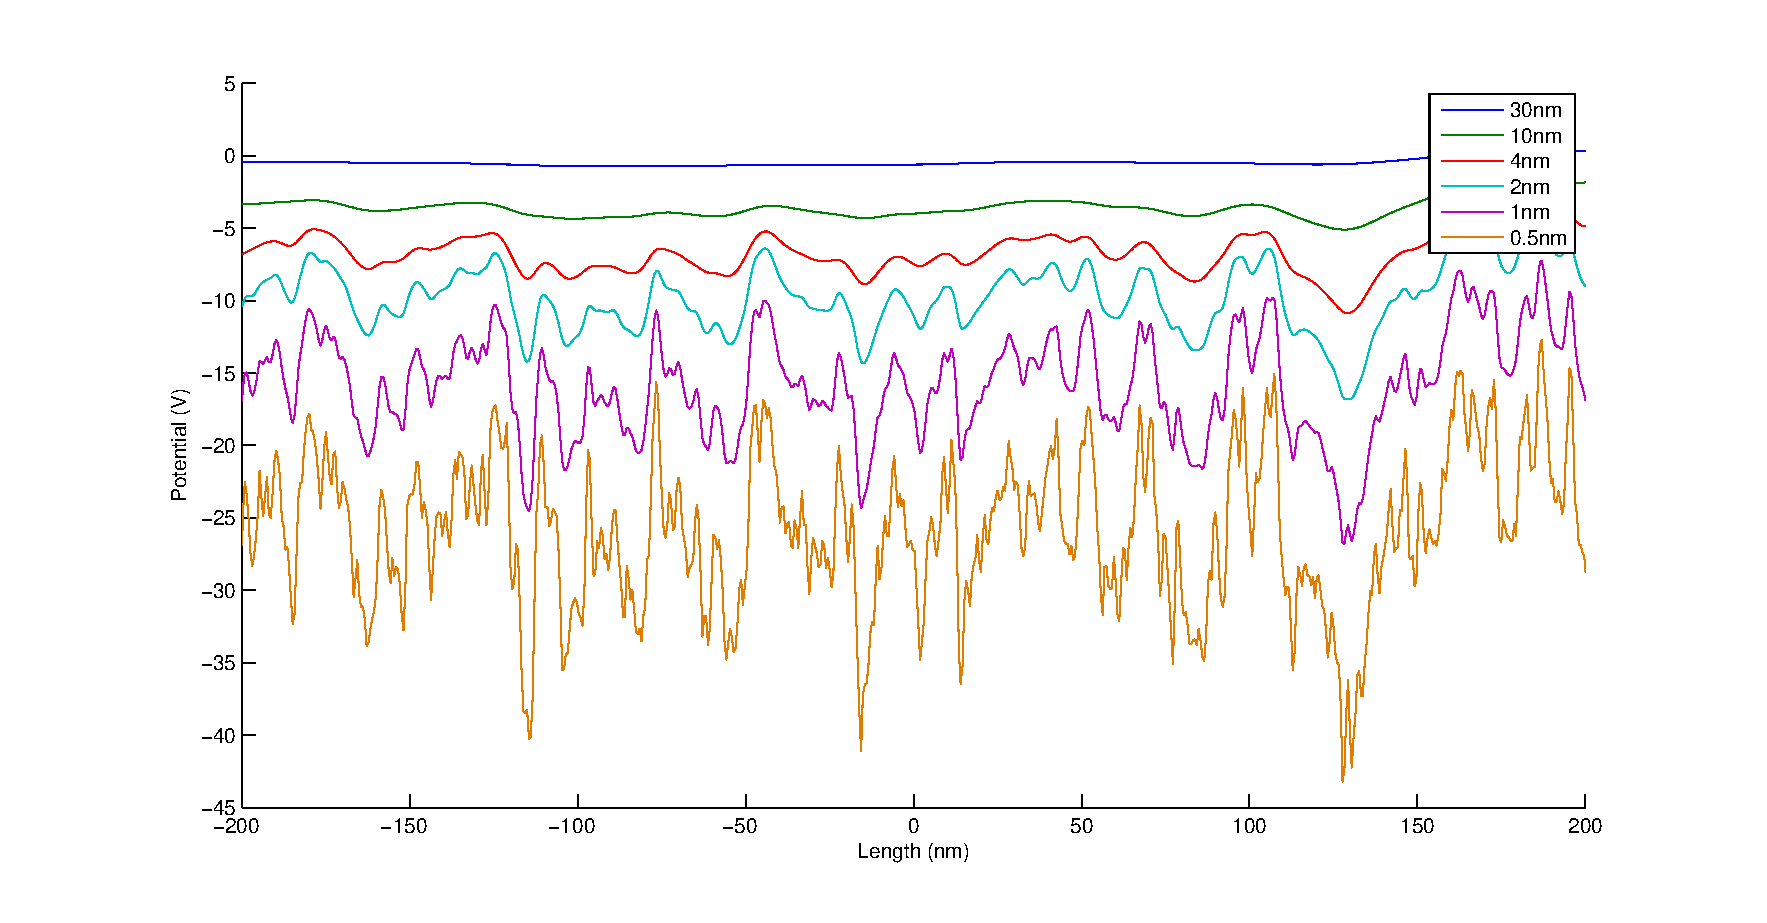
\includegraphics[width=\textwidth]{potentials.eps}
\caption{Movement of branching points in a living \emph{P. Imperitor} (a-c) at 0,1 and 2 months respectively.
Computer simulation with e being the starting and e and f being after 30,000 and 50,000 iterations \label{branching}}
\end{figure}

\begin{figure}
\centering
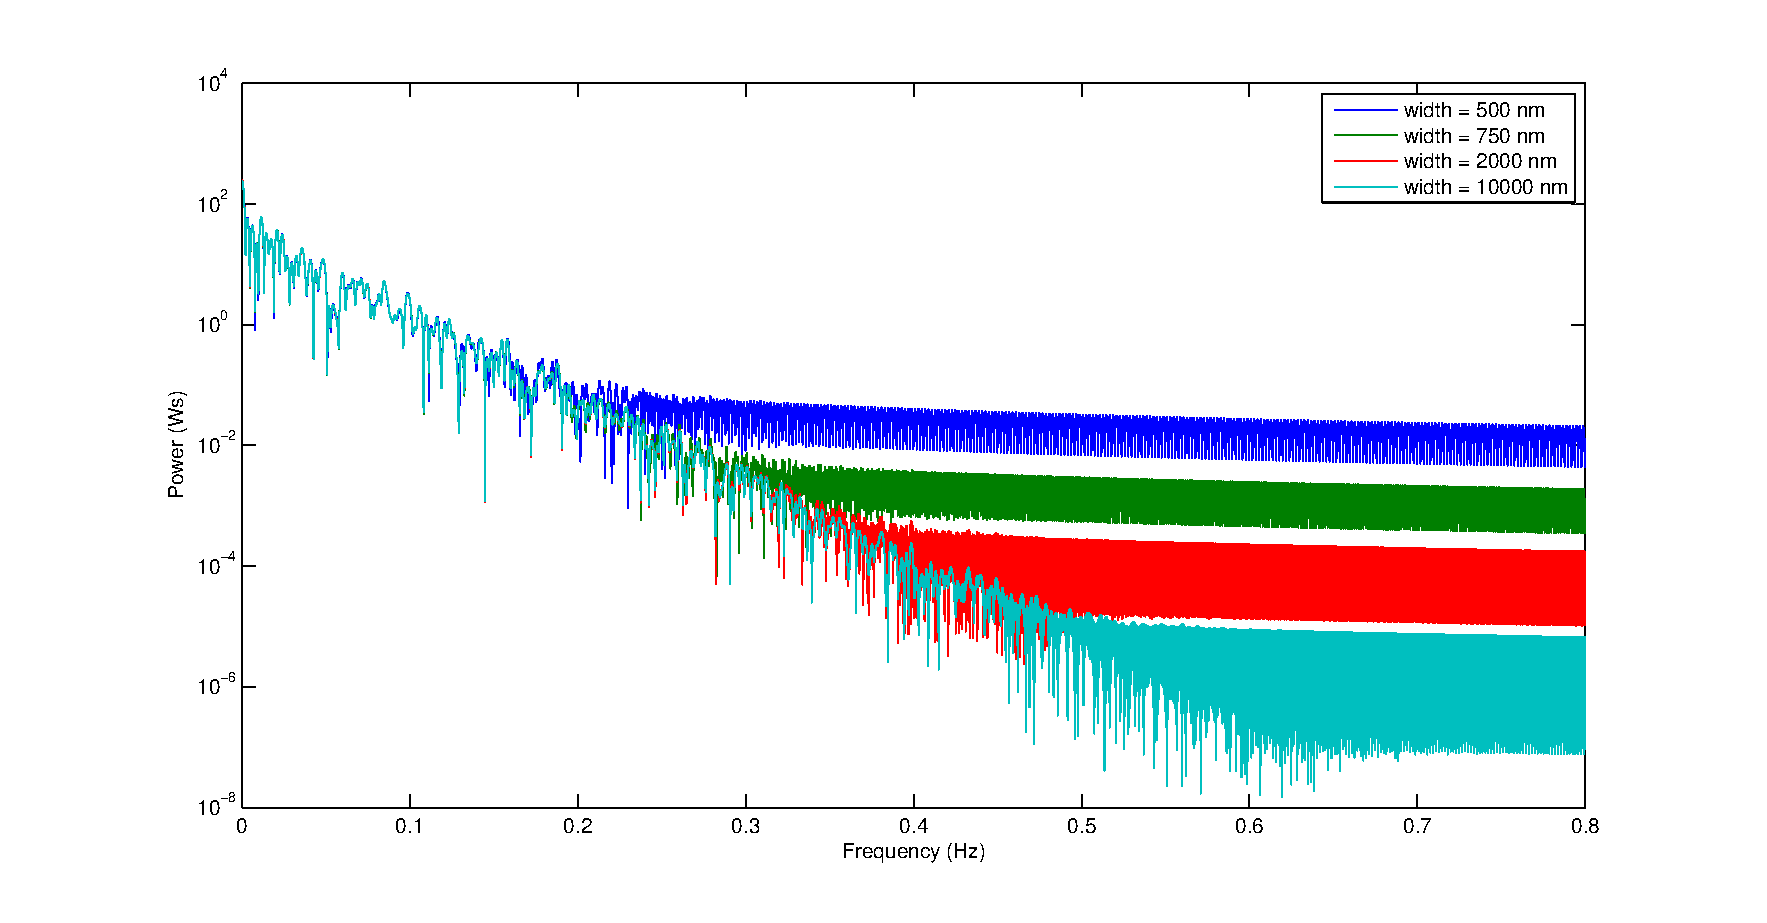
\includegraphics[width=\textwidth]{Fouriers_with_varying_range.eps}
\caption{Movement of branching points in a living \emph{P. Imperitor} (a-c) at 0,1 and 2 months respectively.
Computer simulation with e being the starting and e and f being after 30,000 and 50,000 iterations \label{branching}}
\end{figure}

\begin{figure}
\centering
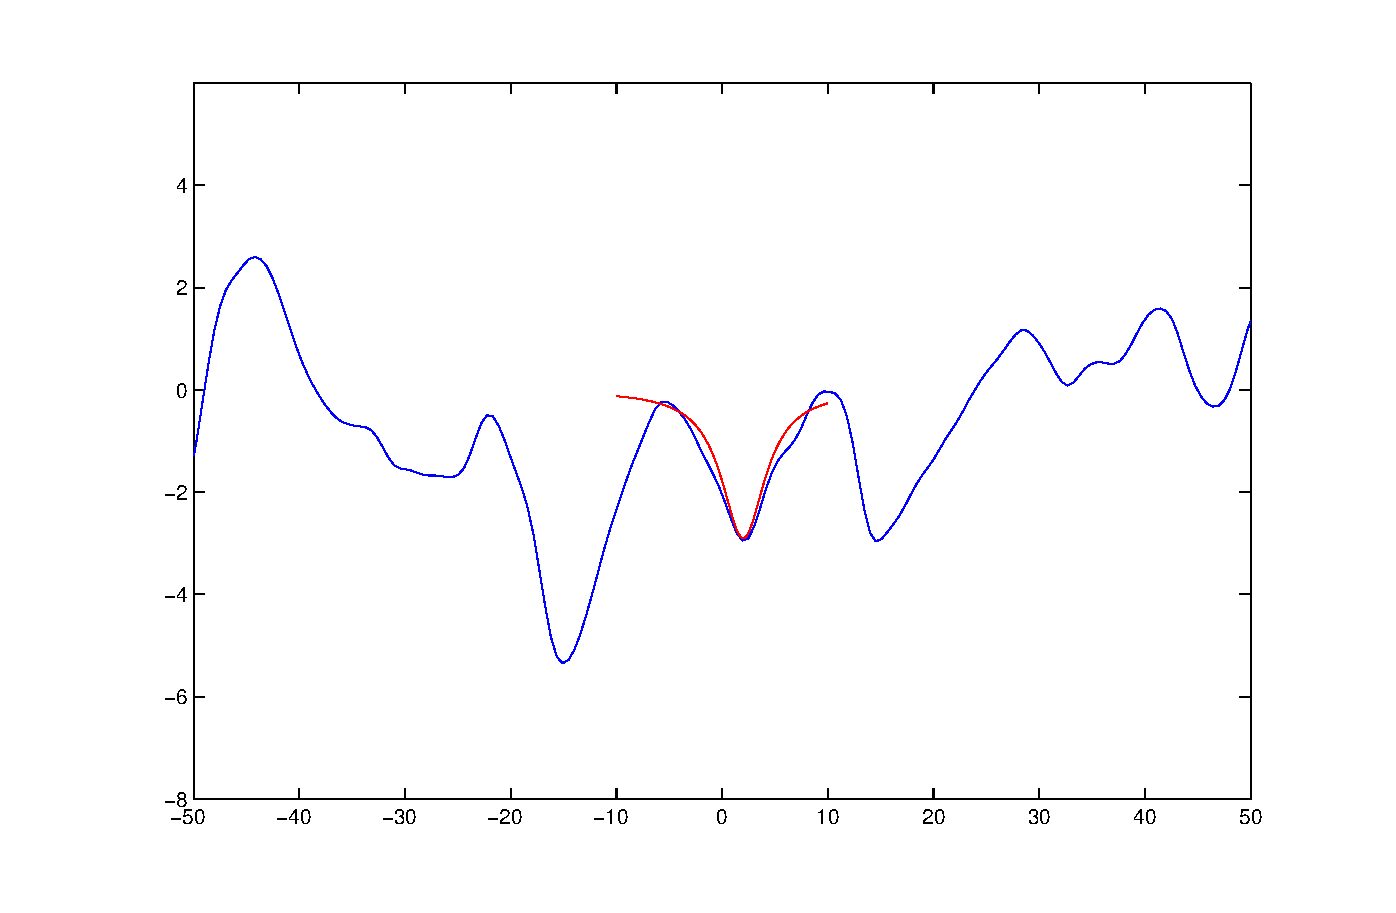
\includegraphics[width=\textwidth]{lorentzianOnLandscape.eps}
\caption{Movement of branching points in a living \emph{P. Imperitor} (a-c) at 0,1 and 2 months respectively.
Computer simulation with e being the starting and e and f being after 30,000 and 50,000 iterations \label{branching}}
\end{figure}

\begin{figure}
\centering
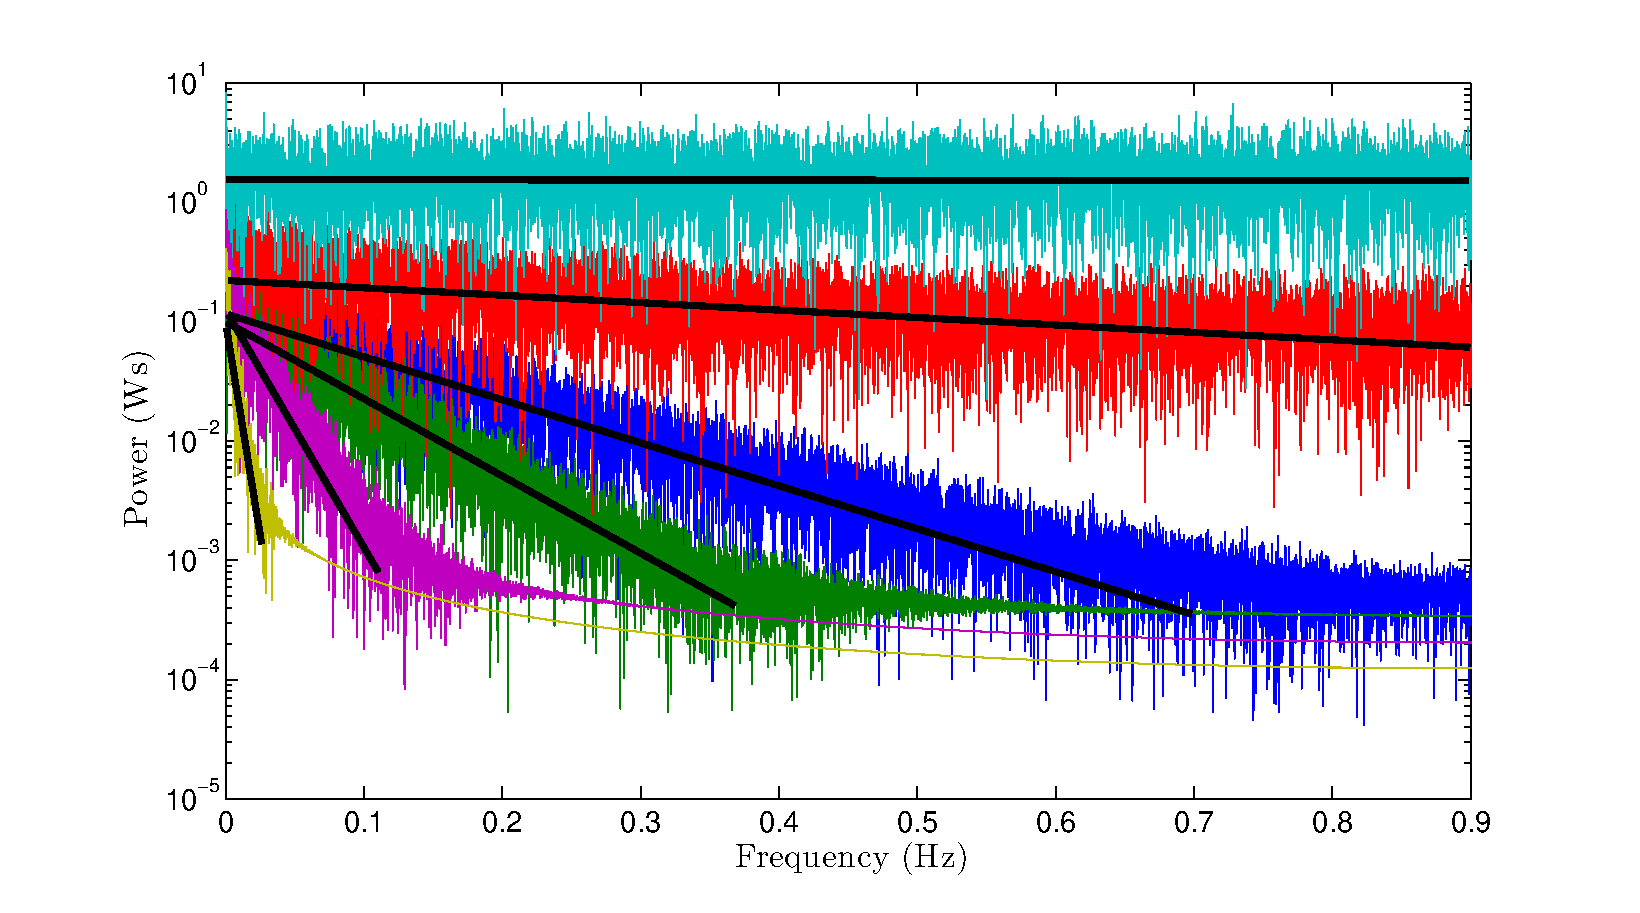
\includegraphics[width=\textwidth]{Fourier_plots_with_varying_d.eps}
\caption{Movement of branching points in a living \emph{P. Imperitor} (a-c) at 0,1 and 2 months respectively.
Computer simulation with e being the starting and e and f being after 30,000 and 50,000 iterations \label{branching}}
\end{figure}




\begin{figure}
\centering
\begin{tikzpicture}
\def\nuPi{3.1459265}
\node[inner sep=0pt] (russell) at (3,-2)
    {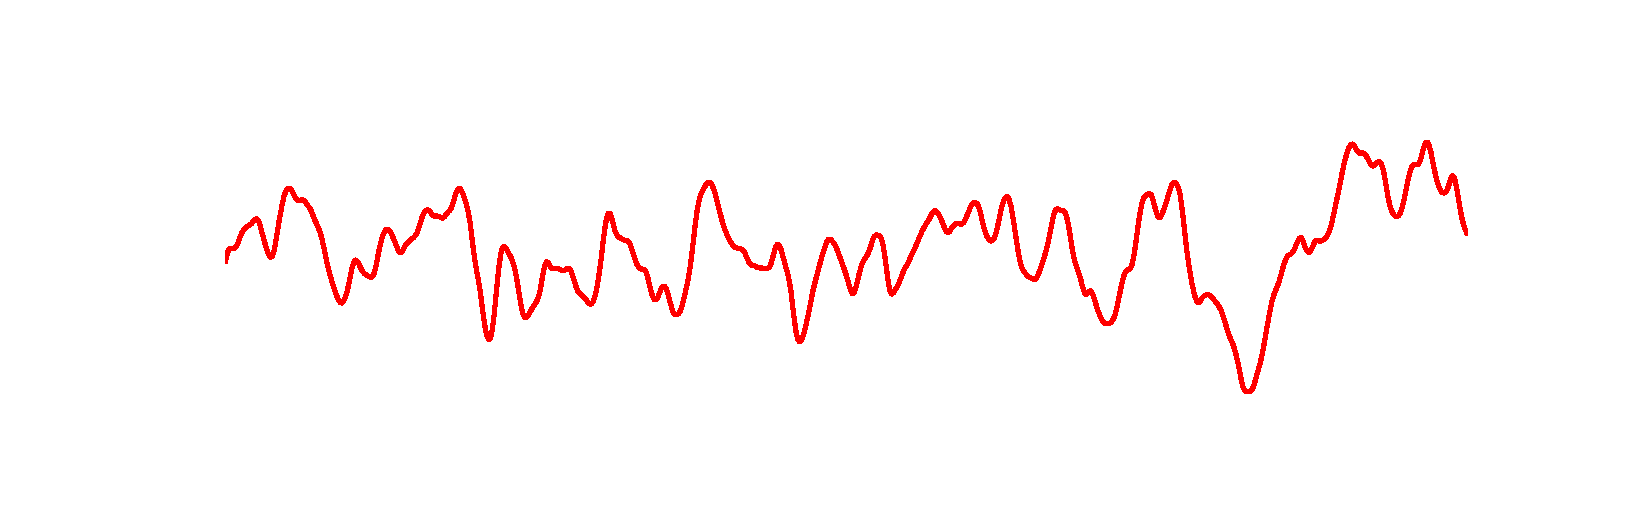
\includegraphics[width=.45\textwidth]{onelandscape.eps}};

\path [fill=mycolor1] (0,0) rectangle (6,1);
\node [white] at (3, 0.5) {p-GaAs};
\draw [thick, ->] (-0.2,0) --(-0.2,-2);
\node [left] at (-0.2,-1) {$d$};
\node [red,right] at (6.2,-2) {Potential};
\foreach \i in {1,2,...,30}{
  \foreach \j in {1,2,3}{
  \pgfmathsetmacro{\dx}{(rand*0.5+0.5)*6}
  \pgfmathsetmacro{\dy}{(rand*0.5+0.5)}
  \pgfmathsetmacro{\rot}{rand*0.1}   
  \shade[ball color=mycolor1] ({\dx+\rot},{-(\dy+\rot)*\j/5}) circle(0.12); 
  }
}
\draw [thick,decorate,decoration={brace,amplitude=2pt,raise=3pt},yshift=0pt]
(6.2,0) -- (6.2,-0.8) node [black,midway,xshift=0.8cm] {donors};

\path [fill=mycolor3] (0,-3) rectangle (6,-3.5);
\path [fill=mycolor3] (0,-4) rectangle (6,-4.5);

\draw [thick, <-] (5.5,-2.5) --(6.5,-3.75);
\draw [thick, <-] (5.5,-3.75) --(6.5,-3.75);
\draw [thick, <-] (5.5,-5) --(6.5,-3.75);
\node [right] at (6.5,-3.75) {i-GaAs};

\draw [thick, <-] (0.5,-3.25) --(-0.5,-3.75);
\draw [thick, <-] (0.5,-4.25) --(-0.5,-3.75);
\node [left] at (-0.5,-3.75) {AlAs};

\path [fill=mycolor2] (0,-6) rectangle (6,-7);
\node [white] at (3, -6.5) {n-GaAs};

\end{tikzpicture}
\end{figure}

\begin{figure}
\centering
\begin{tikzpicture}[scale=2]
\draw [red, thick, dashed] (2,0) --(4,-2);

\draw [thick] (0,0) --(6,0);
\node [below] at (0,-2.1) {$0$};
\node [right] at (6,-2) {$x$};
\draw [thick, |->] (0,-2) --(6,-2);
\node [thick, cross=3pt] at (4,-2) {};
\node [below right] at (4,-2) {$x=x_0$};
\draw [thick, dashed] (4,0) --(4,-2);
\draw (3.75,0) --(3.75,-0.25);
\draw (3.75,-0.25) --(4,-0.25);  
\shade[ball color=mycolor1] (2,0) circle(0.12); 
\draw [thick, ->] (0,0.3) --(2,0.3);
\node [above] at (1,0.3) {$C_i$};
\node [right] at (4,-1) {$d$};
\node [below left] at (3,-1) {$r_i(x_0)$};

\draw [thick,decorate,decoration={brace,amplitude=2pt,raise=3pt},yshift=0pt]
(2.1,0.2) -- (4,0.2) node [black,midway,yshift=0.4cm] {$x_0 - C_i$};

\end{tikzpicture}
\end{figure}

\section{Discussion}

\section{Conclusion}

\section{Summary}

\bibliographystyle{unsrt}
\bibliography{mybib} 

\end{document}

\message{ !name(report.tex) !offset(-413) }
